\documentclass[12pt,a4paper]{article}
\usepackage[utf8]{inputenc}
\usepackage[english]{babel}
\usepackage{amsmath}
\usepackage{amsfonts}
\usepackage{amssymb}
\usepackage{graphicx}

\title{CAGD Exercise 5}
\author{Hanna Huber e0925230\\Stefan Zaufl e0925357}

\begin{document}
\maketitle
\section{Cubic Spline Interpolation of Surfaces}

A data set $(x_i, y_j, f_{ij}), i\in 1...50, j\in 1...50,  f_{ij}\in\mathbb{R}^3$ is generated by adding noise to a smooth function and taking a random sample (see Figure~\ref{fig:sVSp}). These sample points are interpolated using a cubic tensor product spline. \\\\
%
For this purpose, we create an interpolating cubic spline in each dimension by interpolating the points $(x_i, 1, f_{i1}), i\in 1...50$ and $(1, y_j, f_{1j}), j\in 1...50$, yielding the surface boundary curves $s_x$ and $s_y$. \\\\
%
The remaining surface points are determined by calculating the difference vectors $\Delta_{0,t} = \overrightarrow{s_x(0)s_y(t)}, t\in\{0,...,1\}$ and shifting them along the curve $s_x$:
\begin{equation}\label{eq:surfInterpol}
s(t_x, t_y) = s_x(t_x) + \Delta_{0,ty}, \quad  t_x\in\{0,...,1\}, t_y\in\{0,...,1\}
\end{equation}

Comparing the interpolated surface given be Equation~\ref{eq:surfInterpol} to the underlying noisy function (see Figure~\ref{fig:nVSi}) and to the sampled data (see Figure~\ref{fig:sVSi}), only a few outliers can be detected. They result from outliers along the interpolated boundary curves.

\begin{figure}[hbtp]
\centering
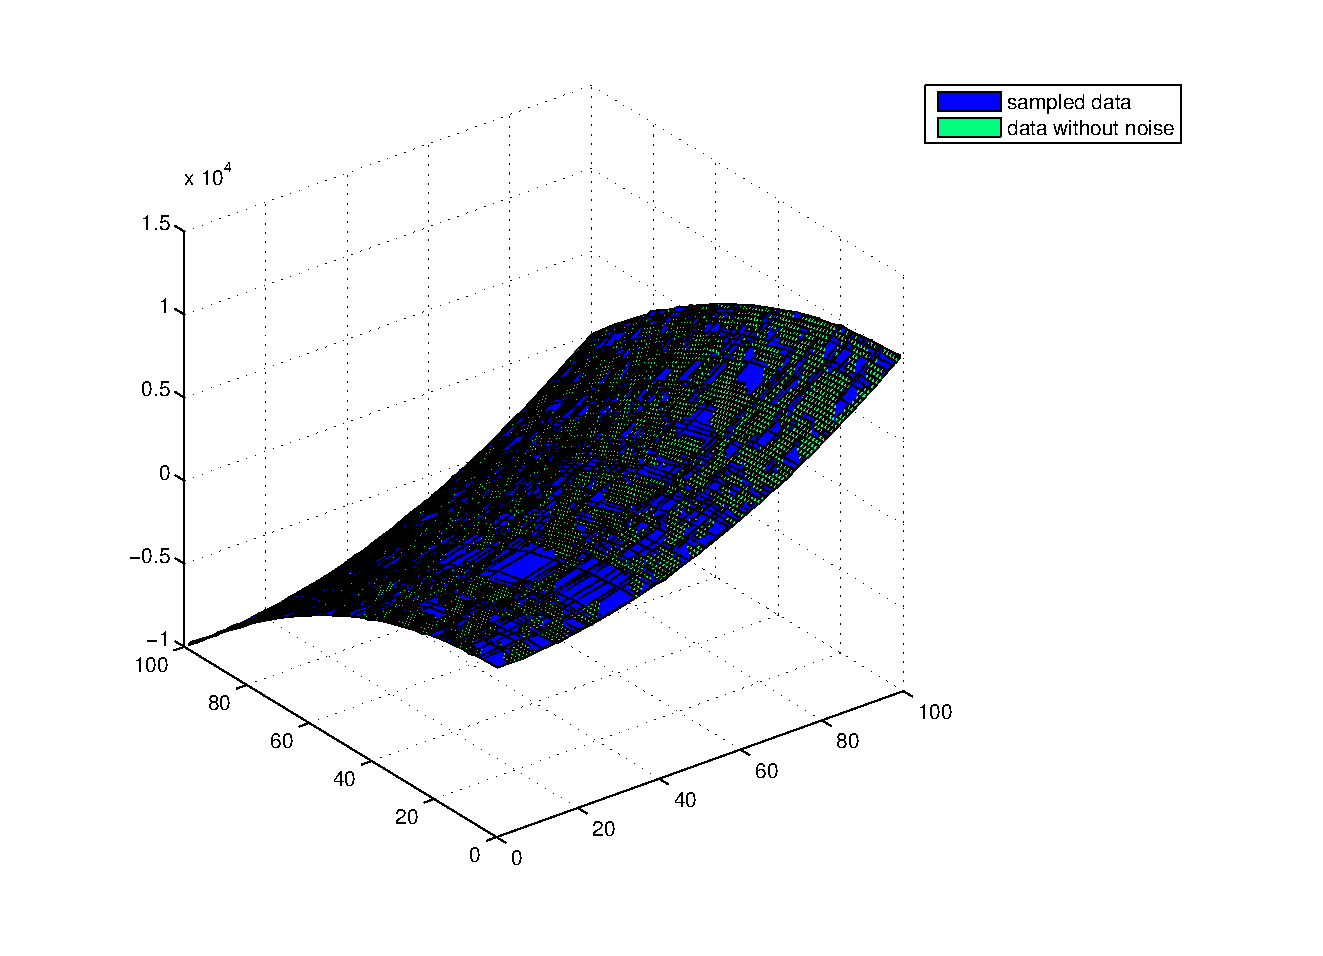
\includegraphics[height=0.4\textheight]{sampledVSPure.eps}
\caption{Comparison of noisy data samples and the underlying smooth function.}
\label{fig:sVSp}
\end{figure}

\begin{figure}[hbtp]
\centering
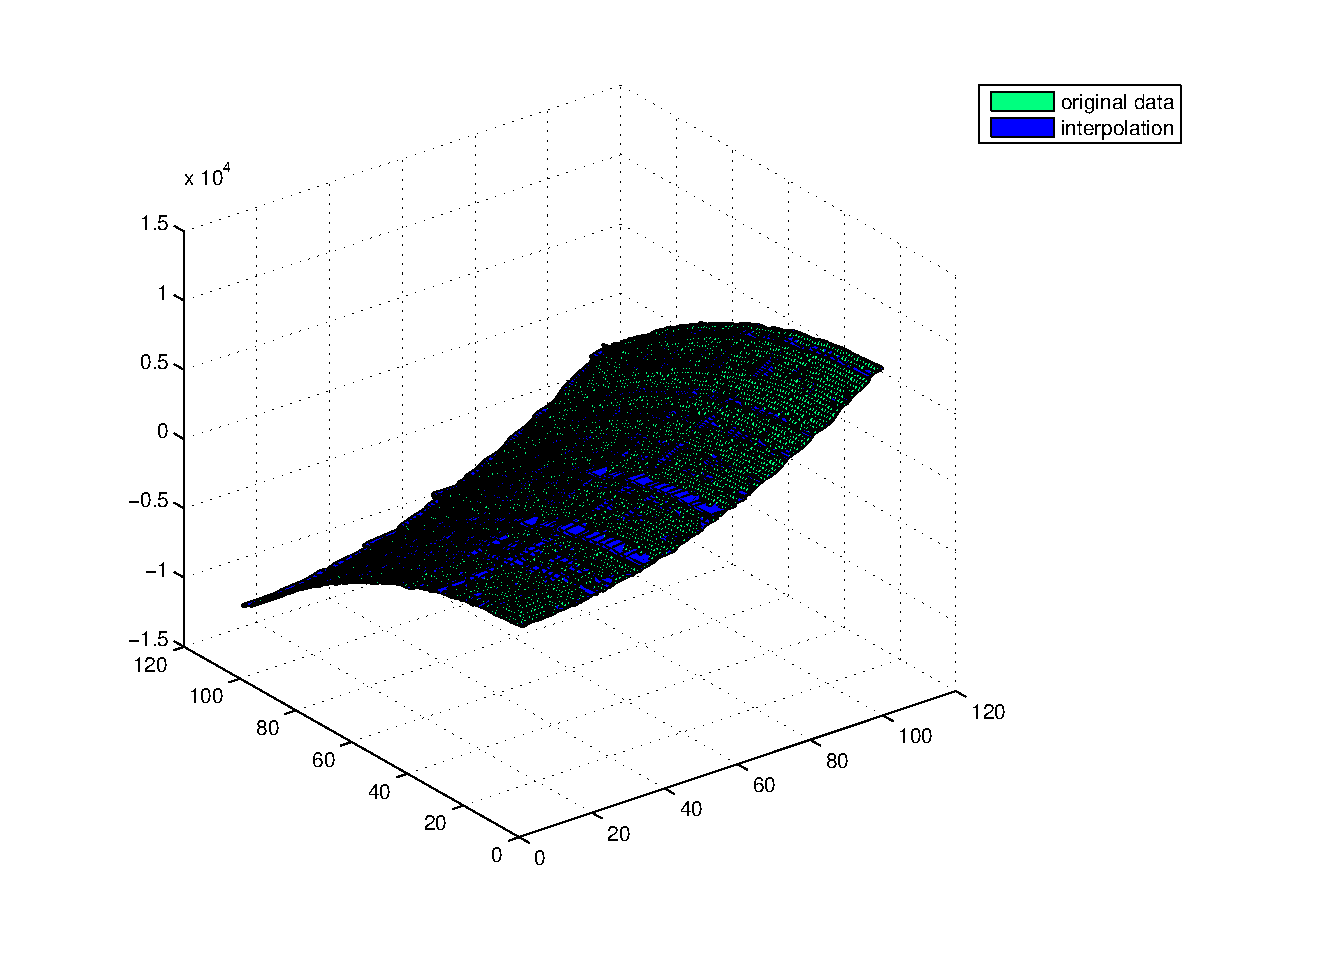
\includegraphics[height=0.45\textheight]{noisyVSInterpol.eps}
\caption{Comparison of noisy function and interpolating surface.}
\label{fig:nVSi}
\end{figure}

\begin{figure}[hbtp]
\centering
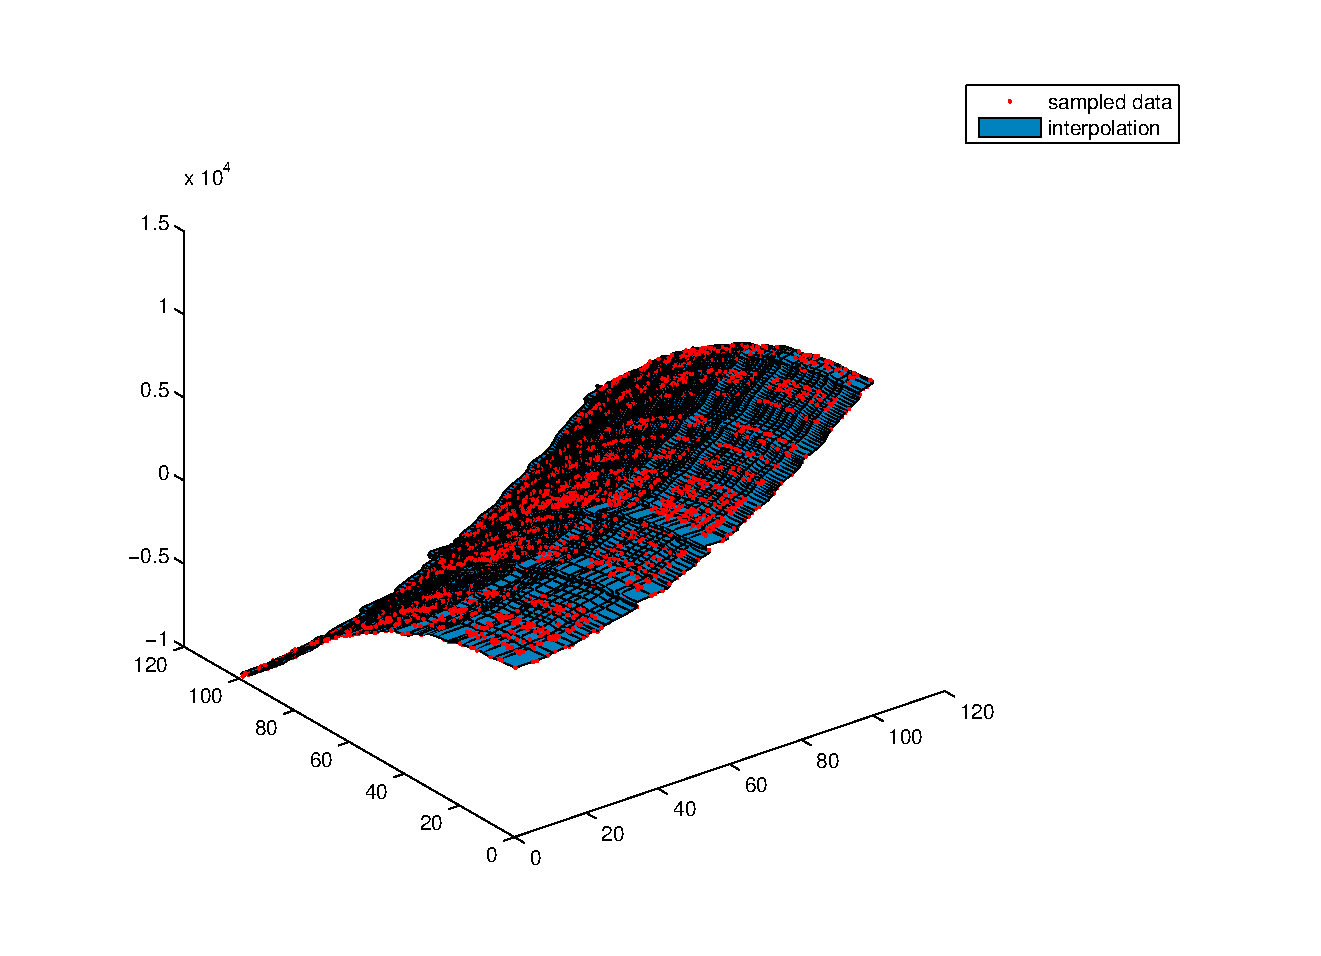
\includegraphics[width=\textwidth]{sampledVSInterpol.eps}
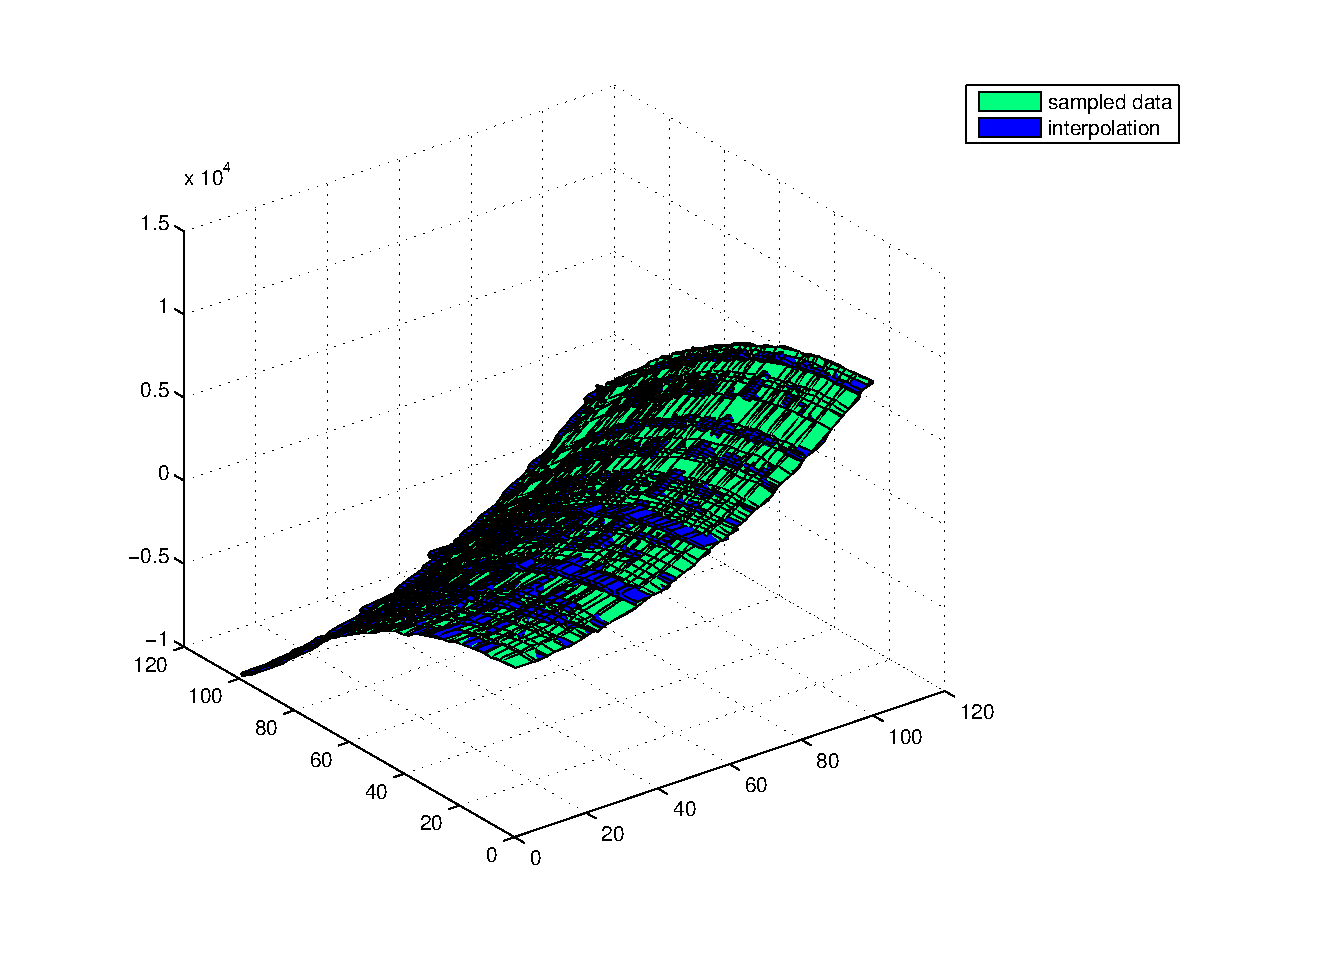
\includegraphics[width=\textwidth]{sampledVSInterpolSurf.eps}
\caption{Comparison of noisy data samples (above: point representation; below: surface representation) and  interpolating surface.}
\label{fig:sVSi}
\end{figure}


\section{Cubic Spline Approximation of Surfaces}

In this section, we use the same data set $(x_i, y_j, f_{ij}), i\in 1...50, j\in 1...50,  f_{ij}\in\mathbb{R}^3$ and approximate it with a cubic tensor product spline using the provided Matlab function \textit{fit}. Figure~\ref{fig:aVSi} shows that the resulting surface is clearly smoother.

\begin{figure}[hbtp]
\centering
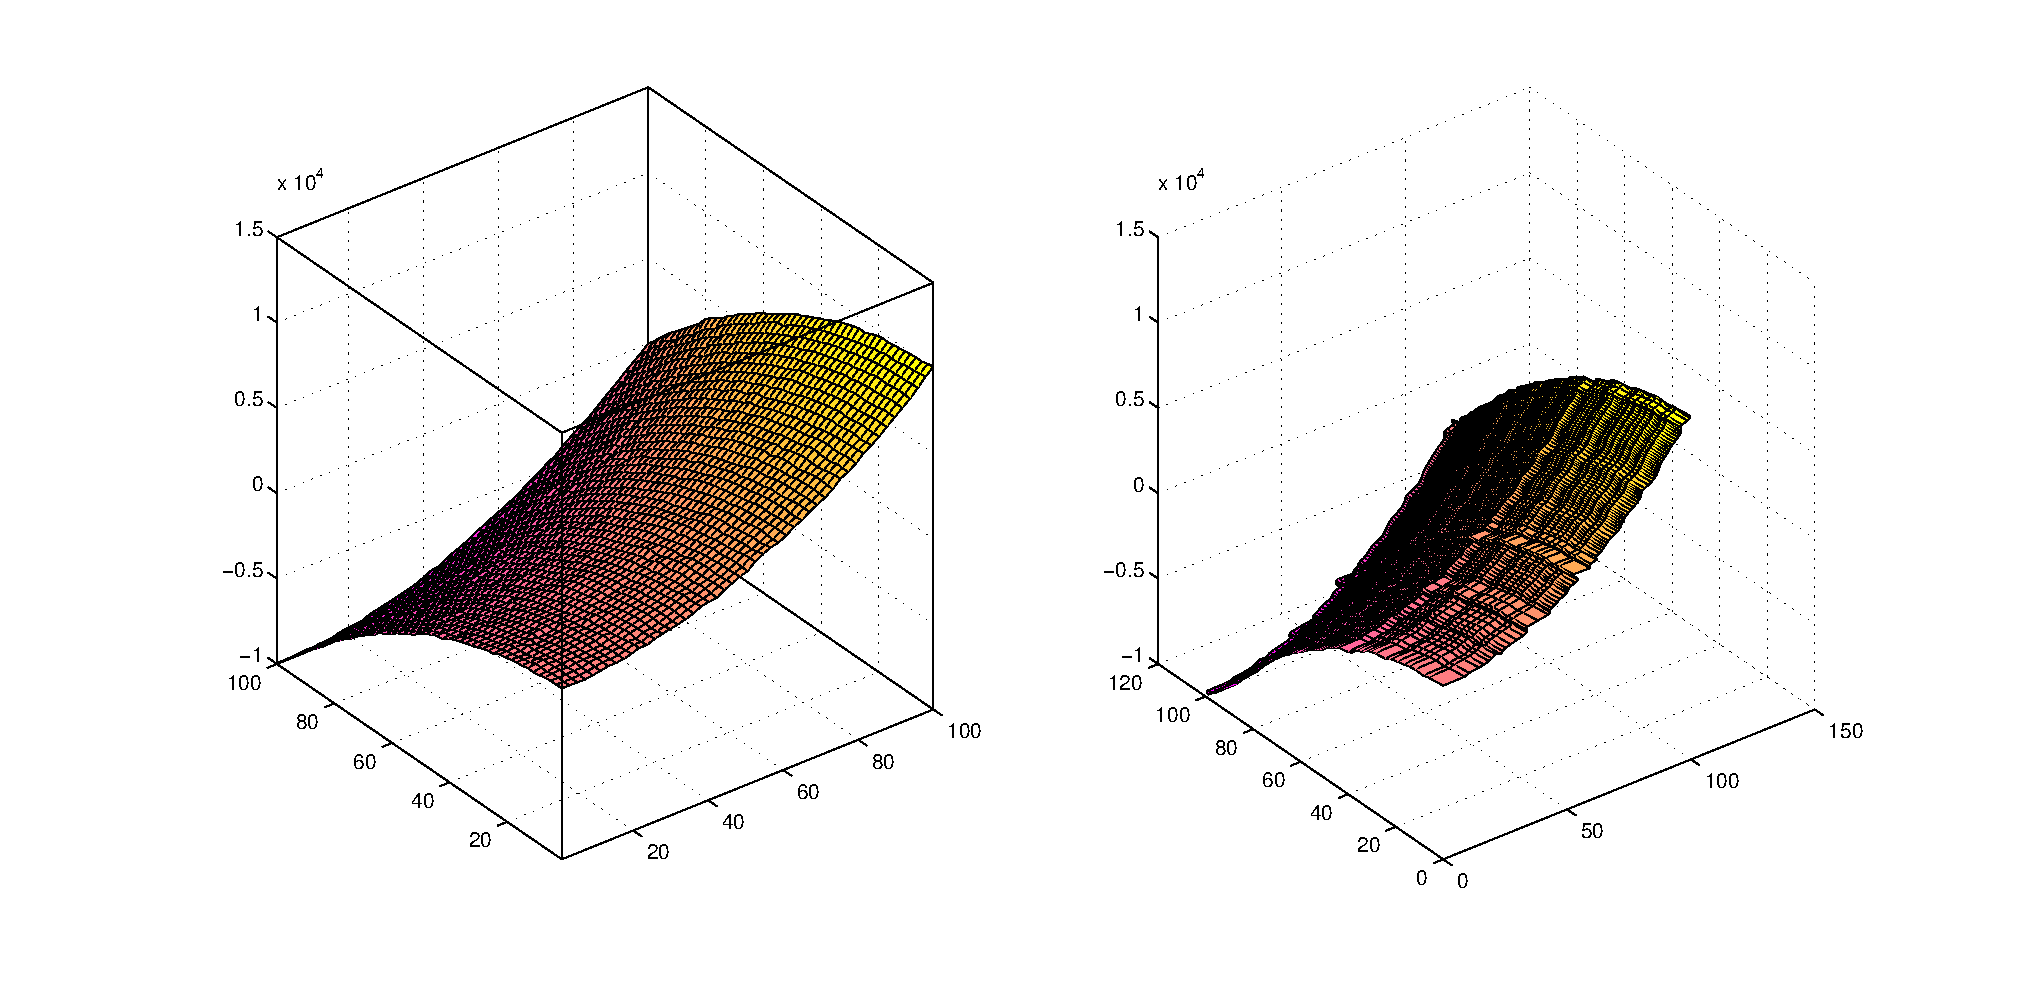
\includegraphics[width=\textwidth]{approxVSInterpol.eps}
\caption{Comparison of noisy data samples and the underlying smooth function.}
\label{fig:aVSi}
\end{figure}

\end{document}